\documentclass[usenames,dvipsnames]{beamer}

\usetheme{Madrid}
\usecolortheme{dolphin}
\setbeamercolor{title}{fg=NavyBlue}
\setbeamercolor{frametitle}{fg=NavyBlue}
\setbeamercolor{section in toc}{fg=NavyBlue}

\usepackage{amsthm}
\usepackage{graphicx}
\usepackage[utf8x]{inputenc}
\usepackage{mathtools}
\mathtoolsset{showonlyrefs}
\usepackage{appendixnumberbeamer}
\usepackage{centernot}
\usepackage{tikz}
\usepackage[lined]{algorithm2e}
\usepackage{caption}
\usetikzlibrary{positioning}
\usepackage{booktabs}
\usepackage{natbib}
\usepackage{appendix}

% ITEMIZE
\settowidth{\leftmargini}{\usebeamertemplate{itemize item}}
\addtolength{\leftmargini}{\labelsep}
\setbeamertemplate{itemize items}[default]
\setbeamertemplate{enumerate items}[default]

\DeclarePairedDelimiter{\abs}{\lvert}{\rvert}
\DeclarePairedDelimiter{\norm}{\|}{\|}
\renewcommand{\Pr}{\mathbb{P}}
\newcommand{\R}{\mathbb{R}}
\newcommand{\Var}{\operatorname{Var}}
\newcommand{\E}{\operatorname{\mathbb{E}}}
\newcommand{\iid}{\ensuremath{\stackrel{\text{iid}}{\sim}}}
\renewcommand{\phi}{\varphi}
\newcommand{\epl}{\varepsilon}
\renewcommand{\d}{\mathrm{d}}
\newcommand{\dd}{\,\mathrm{d}}
\newcommand{\lratext}[1]{\ensuremath{\stackrel{\text{#1}}{\longrightarrow}}}
\newcommand{\toweak}{\rightharpoonup}

% Theorem blocks
\setbeamercolor{block title}{fg=white,bg=NavyBlue}
\newenvironment<>{greenblock}[1][]{%
\setbeamercolor{block title}{fg=white,bg=ForestGreen}%
\begin{block}#2{#1}}{\end{block}}
\newenvironment<>{redblock}[1][]{%
\setbeamercolor{block title}{fg=white,bg=red!75!black}%
\begin{block}#2{#1}}{\end{block}}
\newenvironment<>{orangeblock}[1][]{%
\setbeamercolor{block title}{fg=white,bg=orange!75!black}%
\begin{block}#2{#1}}{\end{block}}
\setbeamercolor{caption name}{fg=NavyBlue}

% Add numbers and take out navigation symbols
\beamertemplatenavigationsymbolsempty
\setbeamercolor{date in head/foot}{fg=gray, bg=white}
\setbeamercolor{author in head/foot}{fg=white,bg=white}
\setbeamercolor{title in head/foot}{fg=white,bg=white}
\setbeamertemplate{footline}{
	\leavevmode%
	\hbox{%
		\begin{beamercolorbox}[wd=.4\paperwidth,ht=2.25ex,dp=1ex,center]{author in head/foot}%
		\end{beamercolorbox}%
		\begin{beamercolorbox}[wd=.3\paperwidth,ht=2.25ex,dp=1ex,center]{title in head/foot}%
		\end{beamercolorbox}%
		\begin{beamercolorbox}[wd=.3\paperwidth,ht=2.25ex,dp=1ex,right]{date in head/foot}%
			\insertframenumber{} / \inserttotalframenumber\hspace*{2ex} 
	\end{beamercolorbox}}%
	\vskip0pt%
}

\definecolor{leg1}{RGB}{0,114,189}
\definecolor{leg2}{RGB}{217,83,25}
\definecolor{leg3}{RGB}{237,177,32}
\definecolor{leg4}{RGB}{126,47,142}
\definecolor{leg5}{RGB}{119,172,48}


% Text starts always from the top of the frame
\newenvironment{frameT}{\begin{frame}[t]}{\end{frame}}

\newcommand*\samethanks[1][\value{footnote}]{\footnotemark[#1]}
\title{Bayesian inference of multiscale differential equations}
\author{Assyr Abdulle \and \underline{Giacomo Garegnani}}
\date{Caltech -- 22 August 2019}
\institute[EPFL]{École polytechnique fédérale de Lausanne \\ \vspace{0.2cm} 
\includegraphics[width=3cm]{Logo-eps-converted-to.pdf}}

\begin{document}

\thispagestyle{empty}
\frame{\titlepage}

\addtocounter{framenumber}{-1}

\begin{frame}
	\frametitle{Short bio}	
	\thispagestyle{empty}
	
	\textbf{Education}
	\begin{itemize}
		\item M.Mus. in Piano at Conservatorio Vivaldi (2012)
		\item B.Sc. in Mathematical Engineering at Politecnico di Milano (2014)
		\item M.Sc. in Computational Science \& Engineering at EPFL (2017)
		\item PhD student in Assyr Abdulle's group at EPFL (since 2017)
	\end{itemize}

	\vspace{0.2cm}
	\textbf{Work experience}
	\begin{itemize}
		\item STMicroelectronics -- R\&D intern (Grenoble, 2015)
		\item MindMaze -- Software Development intern (Lausanne, 2016)
	\end{itemize}
	
	\vspace{0.2cm}
	\textbf{Research interests}
	\begin{itemize}
		\item Probabilistic solvers for differential equations
		\item \underline{Bayesian inference of multiscale differential equations}
	\end{itemize}
\end{frame}

\addtocounter{framenumber}{-1}

\begin{frame}
	\thispagestyle{empty}
	\frametitle{Outline}
	\tableofcontents
\end{frame}

\addtocounter{framenumber}{-1}

\section{Probabilistic solvers for differential equations}

\AtBeginSection[]
{
	\begin{frame}<beamer>
		\thispagestyle{empty}
		\frametitle{Outline}
		\tableofcontents[currentsection]
	\end{frame}
	\addtocounter{framenumber}{-1}
}

\begin{frameT}
	\frametitle{Probabilistic solvers for differential equations}
	
	{\color{NavyBlue}Main idea:} Design numerical solvers for differential equations which account for errors in a probabilistic/statistical manner
	
	\vspace{0.3cm}
	\only<1>{
	{\color{NavyBlue} Some contributions:}
	
	{\color{BrickRed} ODEs:} Two families of methods
	\begin{itemize}
		\item From Runge--Kutta methods: \cite{CGS17}, \cite{LSS17}, \cite{AbG18}, (\ldots)
		\item From filtering methods: \cite{CCC16}, \cite{SDH14}, \cite{KeH16}, \cite{KSH18}, (\ldots)
	\end{itemize} 
	
	{\color{ForestGreen} PDEs:} \cite{CGS17}, \cite{COS17, COS17b} (\ldots)}
	
	\only<2-4>{{\color{BrickRed} Motivations:}}
	
	\only<2>{Uncertainty quantification of chaotic equations
	\begin{figure}
		\begin{center}
			\begin{tabular}{c}
				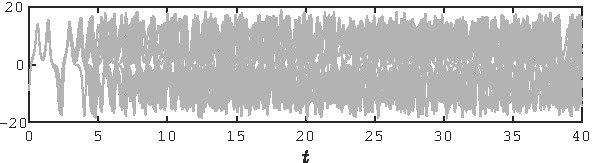
\includegraphics[scale=0.55]{Figures/LorenzTest1} \\
				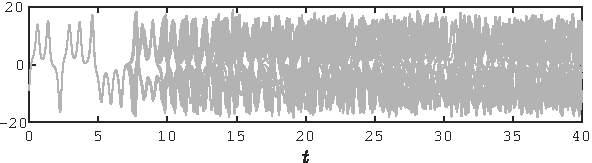
\includegraphics[scale=0.55]{Figures/LorenzTest2} \\
				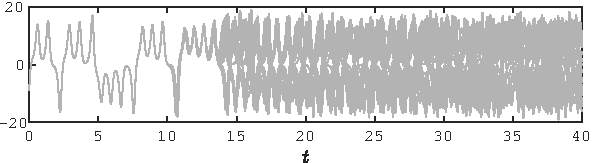
\includegraphics[scale=0.55]{Figures/LorenzTest3}
			\end{tabular}
		\end{center}
		\caption{Solution of the Lorenz system with different perturbations}
	\end{figure}}
	
	\only<3>{A posteriori error estimators
	\begin{figure}
		\begin{center}
			\begin{tabular}{cc}
				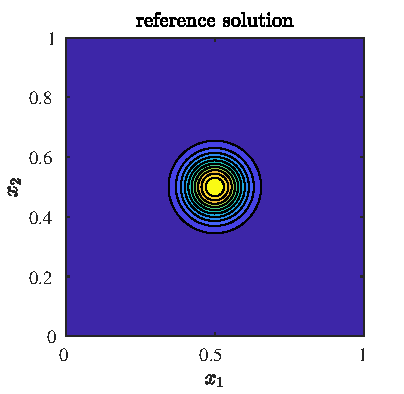
\includegraphics[scale=0.65]{Figures/MeshAdapt2D_ReferenceSol} & 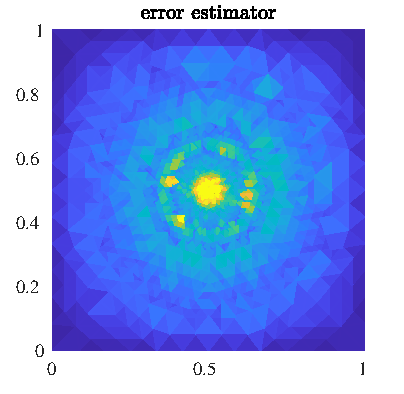
\includegraphics[scale=0.65]{Figures/MeshAdapt2D_ErrEst}
			\end{tabular}
		\end{center}
	\caption{Probabilistic error estimator for a simple elliptic PDE}
	\end{figure}}
	
	\only<4>{Bayesian inverse problems
	\begin{figure}
		\begin{center}
			\begin{tabular}{cc}
				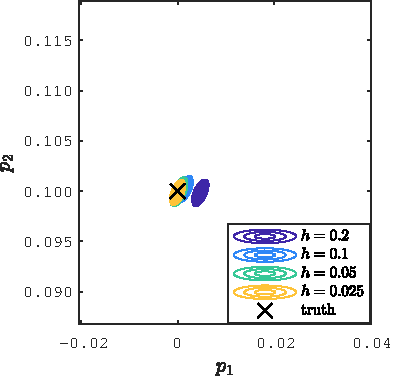
\includegraphics[scale=0.65]{Figures/BayesDet} & 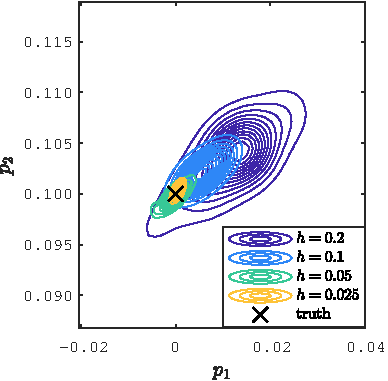
\includegraphics[scale=0.65]{Figures/BayesProb}
			\end{tabular}
		\end{center}
		\caption{Probabilistic correction of posterior distributions.}
	\end{figure}	
	}
\end{frameT}

\subsection{Ordinary differential equations (ODEs)}

\begin{frameT}
	\frametitle{Probabilistic solvers for ODEs}
	{\color{NavyBlue}Notation:} function $f\colon\R^d\to\R^d$, IC $y_0 \in \R^d$ and
	\begin{equation}
	y' = f(y), \quad y(0) = y_0.
	\end{equation}
	{\color{ForestGreen} Exact} and {\color{BrickRed} numerical (Runge--Kutta)} flows
	\begin{equation}
	y(t) = {\color{ForestGreen}\phi_t(y_0)} \lratext{discretization} y_{n+1} = {\color{BrickRed}\Psi_h(y_n)}
	\end{equation}
	 
	\only<2>{{\color{NavyBlue}Additive noise method (AN-RK) (\cite{CGS17})}  
	
	Stochastic process $\{Y_n\}_{n=1, 2, \ldots}$ with recurrence
	\begin{equation}
	Y_{n+1} = \underbrace{\color{BrickRed}\Psi_h(Y_n)}_{\text{deterministic}} + \underbrace{\xi_n(h)}_{\text{random}}.
	\end{equation}
	{\color{BrickRed} Main assumption}: For $p > 1$ and $Q \in \R^{d\times d}$
	\begin{equation}
	\xi_n(h) \iid \mathcal N(0, Qh^{2p+1}).
	\end{equation}
	}
	
	\only<3>{{\color{NavyBlue}Random time step method (RTS-RK) (\cite{AbG18})}
	\begin{equation}
	Y_{n+1} = \Psi_{{\color{NavyBlue} H_n}}(Y_n),
	\end{equation}
	{\color{BrickRed}Main assumption}: $\{H_n\}_{n=0,1,\ldots}$ iid such that for $h, C > 0$ and $p > 1$
	\begin{equation}
	H_n > 0 \text{ a.s.}, \quad \E H_n = h, \quad \Var H_n = Ch^{2p + 1}.
	\end{equation} 
	Example: $H_n \iid \mathcal{U}(h-h^{p+1/2}, h+h^{p+1/2})$.
	}
\end{frameT}

\begin{frame}
	\frametitle{Probabilistic solvers for ODEs -- Properties}
	
	{\color{BrickRed} Assumptions:} 
	\begin{itemize}
		\item RK method of order $q$
		\item variance of random perturbations $\propto h^{2p+1}$
	\end{itemize}
	
	\vspace{0.5cm}
	{\color{NavyBlue}Properties:}
	
	Common to AN-RK and RTS-RK
	\begin{itemize}
		\item {\color{ForestGreen} Strong convergence:} $\E\norm{y(hn)-Y_n} \leq Ch^{\min\{p, q\}}$
		\item {\color{ForestGreen} Weak convergence:} $\abs{\Phi\big(y(hn)\big) - \E\Phi(Y_n)} \leq Ch^{\min\{2p, q\}}$, $\Phi$ smooth
		\item Good qualitative behaviour for {\color{ForestGreen} Bayesian inference problems}
	\end{itemize}
	
	\vspace{0.2cm}
	Only for RTS-RK: Geometric properties
	\begin{itemize}
		\item Conservation of {\color{ForestGreen}first integrals} (e.g., mass in chemical reactions)
		\item Good approximation for {\color{ForestGreen}Hamiltonian problems} over long time spans
	\end{itemize}
\end{frame}

\begin{frame}
	\frametitle{Probabilistic solvers for ODEs --  Numerical example}
	\only<1>{Hénon--Heiles system (celestial dynamics), {\color{ForestGreen}energy}
	\begin{equation}\label{eq:HamHH}
	{\color{ForestGreen}E(v, w)} = \frac{1}{2}\norm{v}^2 + \frac{1}{2}\norm{w}^2 + w_1^2w_2 - \frac{1}{3}w_2^3.
	\end{equation}
	Hamiltonian ODE ($y = (v, w)^\top$)
	\begin{equation}
	\begin{alignedat}{2}
		v'(t) &= -\partial_w {\color{ForestGreen}E(v, w)}, &&\quad v(0) = v_0, \\
		w'(t) &= \partial_v {\color{ForestGreen}E(v, w)}, &&\quad w(0) = w_0.
	\end{alignedat}
	\end{equation}
	
	{\color{BrickRed} Base numerical solver:} Störmer--Verlet method (symplectic)
	
	\vspace{0.3cm}	
	{\color{NavyBlue} Goal:} Determine posterior distribution over $(v_0, w_0)$ given noisy observations of $y(t)$ and prior information on the unknown}

	\only<2>{
	
	\begin{figure}
		\begin{center}
			\begin{tabular}{cc}
				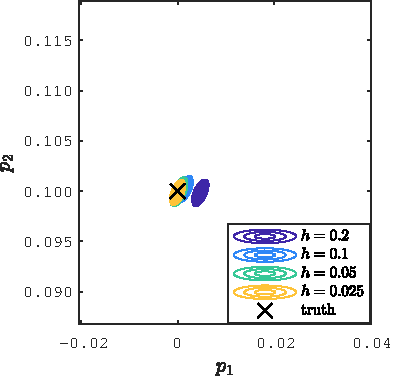
\includegraphics[scale=0.75]{Figures/BayesDet} & 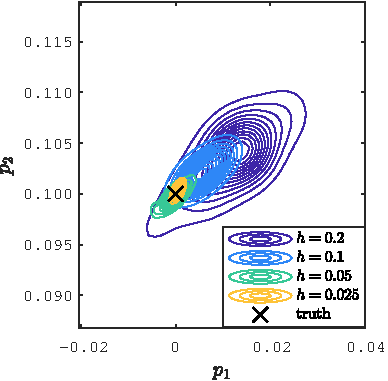
\includegraphics[scale=0.75]{Figures/BayesProb}
			\end{tabular}
		\end{center}
		\caption{Left: deterministic Störmer--Verlet. Right: RTS-RK with Störmer--Verlet \\ Posterior variance reflects the uncertainty due to numerical discretization.}
	\end{figure}
	}
\end{frame}

\subsection{Elliptic partial differential equations (PDEs)}

\begin{frameT}
\frametitle{Probabilistic solvers for PDEs}
{\color{NavyBlue}Notation:} domain $\Omega \subset \R^d$, rhs $f \colon \Omega \to \R$, BC $g \colon \partial \Omega \to \R$, elliptic tensor $A \colon \Omega \to \R^{d\times d}$, equation
\begin{equation}
\begin{aligned}
-\nabla \cdot (A \nabla u) &= f, &&\text{in } \Omega,\\
u &= g, &&\text{on } \partial \Omega,
\end{aligned}
\end{equation}
\only<2-3>{{\color{ForestGreen}Weak formulation:} find $u \in V \equiv H^1_0(\Omega)$ such that
\begin{equation}
	\int_\Omega A \nabla u \cdot \nabla v = \int_\Omega fv, \quad \forall v \in V.
\end{equation}
}
\only<3>{{\color{BrickRed} Galerkin projection:} find $u_h \in V_h \subset V$, $\dim V_h < \infty$ such that
\begin{equation}
	\int_\Omega A \nabla u_h \cdot \nabla v_h = \int_\Omega fv_h, \quad \forall v_h \in V_h.
\end{equation}
{\color{BrickRed} Linear FEM:} Choose $V_h = \{\text{Piecewise linear fcts. on mesh } \mathcal{T}_h \text{ of } \Omega\}$
}
\end{frameT}

\begin{frame}
\frametitle{Probabilistic solvers for PDEs}
	
{\color{NavyBlue} Idea:} In RTS-RK randomization of time steps \\ $\implies$ (controlled) randomization of the mesh $\mathcal T_h$: move vertices with random perturbations $\propto h^p$

\vspace{0.3cm}
{\color{NavyBlue} Properties: (partially WIP)}
\begin{itemize}
	\item {\color{ForestGreen}A priori convergence} of FEM still applies (in a strong sense)
	\item New angle on {\color{ForestGreen} a posteriori convergence} of FEM: employ variability on nodes as an error indicator $\implies$ mesh adaptivity! 
	\item Same advantages on {\color{ForestGreen} Bayesian inference problems} as in ODE case
\end{itemize}
\end{frame}

\begin{frame}
\frametitle{Probabilistic solvers for PDEs -- Numerical example}
\begin{figure}
	\centering
	\begin{tabular}{cc}
		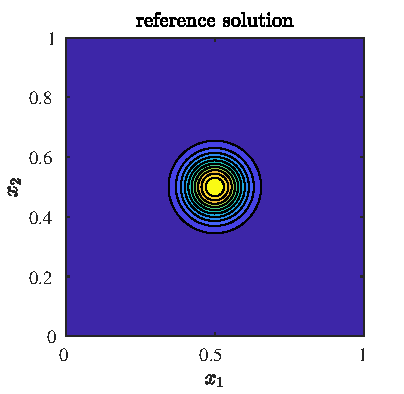
\includegraphics[scale=0.55]{Figures/MeshAdapt2D_ReferenceSol} & 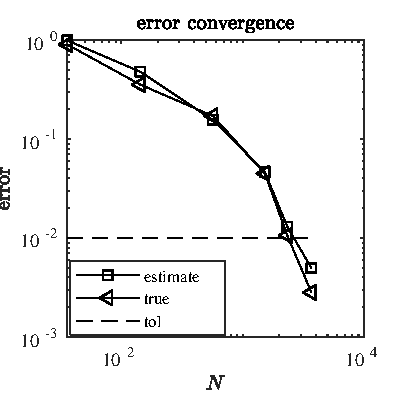
\includegraphics[scale=0.55]{Figures/MeshAdapt2D_ErrConv} \\
		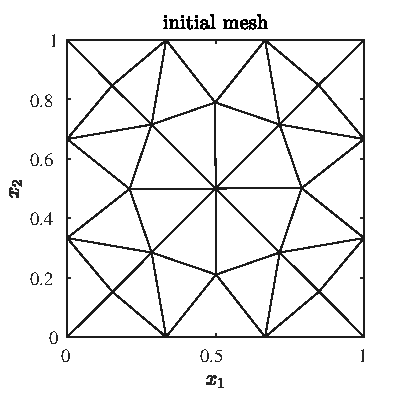
\includegraphics[scale=0.55]{Figures/MeshAdapt2D_InitMesh} & 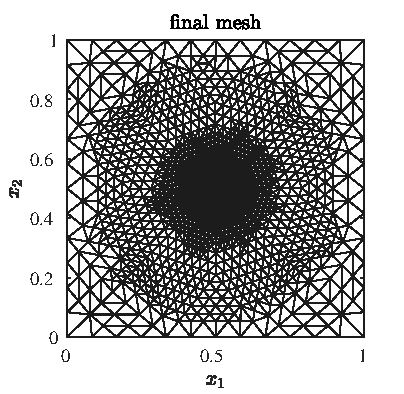
\includegraphics[scale=0.55]{Figures/MeshAdapt2D_FinalMesh}\\
	\end{tabular}
	\caption{Mesh adaptivity based on probabilistic error estimators for a simple PDE}
\end{figure}
\end{frame}

\begin{frame}
\frametitle{Probabilistic solvers for PDEs -- Numerical example}
\begin{figure}
	\centering
	\begin{tabular}{cc}
		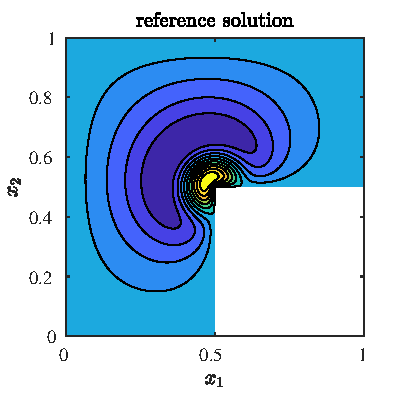
\includegraphics[scale=0.55]{Figures/MeshAdapt2D_2_ReferenceSol} & 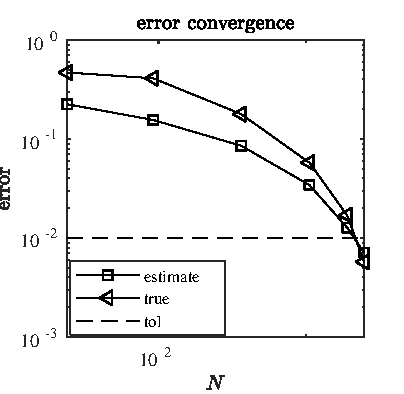
\includegraphics[scale=0.55]{Figures/MeshAdapt2D_2_ErrConv} \\
		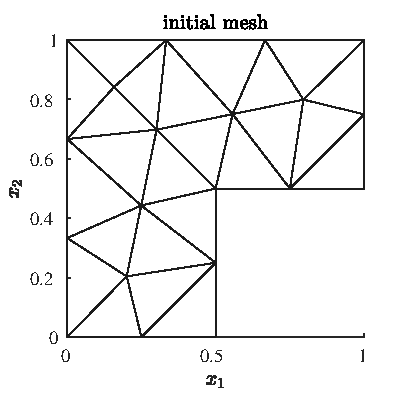
\includegraphics[scale=0.55]{Figures/MeshAdapt2D_2_InitMesh} & 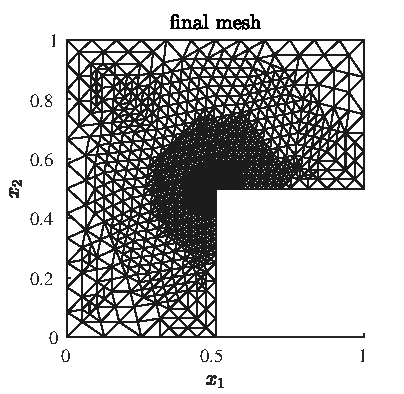
\includegraphics[scale=0.55]{Figures/MeshAdapt2D_2_FinalMesh}\\
	\end{tabular}
	\caption{Mesh adaptivity based on probabilistic error estimators for a simple PDE}
\end{figure}
\end{frame}


\section{Bayesian inference of multiscale differential equations}

\begin{frame}
	\frametitle{Motivation}
	
	\begin{minipage}[t]{0.49\linewidth}	
	\begingroup \color{BrickRed}
	\begin{center} Bayesian inference \end{center}
		\begin{itemize}
			\item Fit model to data
			\item Full UQ approach 
		\end{itemize}
	\endgroup
	\end{minipage}
	\begin{minipage}[t]{0.49\linewidth}	
	\begingroup \color{NavyBlue}
	\begin{center} Differential equations \end{center}
	\begin{itemize}
		\item Modelling of both deterministic and stochastic problems
		\item Well-developed analysis
	\end{itemize}
	\endgroup
	\end{minipage}

	\vspace{1cm}
	\begin{center}
	\begin{minipage}[t]{0.49\linewidth}	
	\begingroup \color{ForestGreen}
	\begin{center} Multiscale \end{center}
	\begin{itemize}
		\item Numerous real-world applications
		\item Theory of homogenization applies
	\end{itemize}
	\endgroup
	\end{minipage}
	\end{center}
\end{frame}

\subsection{Elliptic PDEs}

\begin{frameT}
	\frametitle{Multiscale elliptic PDEs}
	{\color{NavyBlue}Setting:} domain $\Omega \subset \R^d$, rhs $f \colon \Omega \to \R$, BC $g \colon \partial \Omega \to \R$, elliptic multiscale tensor $A^\epl_u \colon \Omega \to \R^{d\times d}$
	\begin{equation}
	\left\{
	\begin{alignedat}{2}
		- \nabla \cdot ( A^\epl_u \nabla p^\epl) &= f, &&\quad \text{ in } \Omega, \\
		p^\epl &= g, &&\quad \text{ on } \partial \Omega.
	\end{alignedat}
	\right.
	\end{equation}
	The function $u\in X$, $X$ Hilbert, parametrizes the slow variations of $A_u^\epl$.
	
	\vspace{0.3cm}
	\only<2>{{\color{BrickRed}Example:} One dimensional case
	\begin{equation}
		A^\epl_u(x) = C e^{u(x)}\left(2 + \sin\left(\frac{x}{\epl}\right)\right),
	\end{equation}
	where $C > 0$ and $u(x)$ could be smooth (e.g. $u(x) = \sin(x)$) or just $L^2$ (e.g. piecewise constant).
	}
	\only<3>{{\color{ForestGreen}Theory of homogenization:}
	There exist non-oscillating $A^0_u$ such that 
	\[ p^{\varepsilon} \toweak p^0 \text{ in } H^1(\Omega), \]
	where $p^0$ is the solution of
	\begin{equation}
	\left\{
	\begin{alignedat}{2}
		- \nabla \cdot ( A_u^0 \nabla p^0) &= f, &&\quad \text{ in } \Omega, \\
		p^0 &= g, &&\quad \text{ on } \partial \Omega.
	\end{alignedat}
	\right.
	\end{equation}
	}
\end{frameT}

\begin{frameT}
	\frametitle{Multiscale elliptic PDEs}
	
	{\color{NavyBlue} Numerical discretization:} Consider multiscale and homogenized equations
	\begin{minipage}{0.49\linewidth}
	\begin{equation}
	\left\{
	\begin{alignedat}{2}
		- \nabla \cdot ( A^\epl_u \nabla p^\epl) &= f, &&\quad \text{ in } \Omega, \\
		p^\epl &= g, &&\quad \text{ on } \partial \Omega.
	\end{alignedat}
	\right.
	\end{equation}
	{\color{ForestGreen} Pro:} Data $A_u^\epl$ is available \\
	{\color{BrickRed} Con:} necessary {\color{BrickRed}$h \ll \epl$} in FEM
	\end{minipage}
	\begin{minipage}{0.49\linewidth}
	\begin{equation}
	\left\{
	\begin{alignedat}{2}
	- \nabla \cdot ( A_u^0 \nabla p^0) &= f, &&\quad \text{ in } \Omega, \\
	p^0 &= g, &&\quad \text{ on } \partial \Omega.
	\end{alignedat}
	\right.
	\end{equation}
	{\color{ForestGreen} Pro:} Cheap to solve numerically \\
	{\color{BrickRed} Con:} $A^0_u$ is unknown (only existence)
	\end{minipage}
	
	\vspace{0.8cm}	
	\only<2>{{\color{NavyBlue}FE-HMM (\cite{AEE12}):} Numerical method for computing $p^0$
		
	\vspace{0.2cm}
	{\color{ForestGreen} Main idea:} Approximate $A_u^0$ on some points in $\Omega$ employing elliptic micro problems. Convergence properties well-established (\cite{Abd05b})
	
	\vspace{0.2cm}
	{\color{ForestGreen} Take-home message:} There exist computational tools which allow to compute cheaply $p^0$ given the multiscale tensor $A^\epl_u$
	}	
\end{frameT}

\begin{frameT}
	\frametitle{Multiscale elliptic PDEs -- Inverse problems}
	
	\vspace{0.6cm}
	{\color{NavyBlue} General formulation}
	\begin{equation}
		\text{Find } {\color{BrickRed}u \in X} \text{ given observations } y = {\color{ForestGreen}\mathcal{G}^\epl}(u) + \eta \in Y,
	\end{equation}
	
	\only<1>{\begin{itemize}
		\item $X, Y$ Hilbert spaces, $\dim(Y) < \infty$
		\item $\eta \sim \mathcal{N}(0,\Gamma)$, $\Gamma$ covariance operator on $Y$
		\item ${\color{ForestGreen}\mathcal{G}^\epl} \colon X \to Y$ forward operator associated to multiscale elliptic PDE
		\begin{equation}
		\left\{
			\begin{alignedat}{2}
			- \nabla \cdot ( A^\epl_{\color{BrickRed} u} \nabla p^\epl) &= f, &&\quad \text{ in } \Omega, \\
			p^\epl &= g, &&\quad \text{ on } \partial \Omega.
			\end{alignedat}
		\right.
		\end{equation}
	\end{itemize}
	}
	\only<2>{{\color{NavyBlue} Bayesian interpretation:} Given prior $\mu_{\mathrm{pr}}$ on $X$, find posterior $\mu^\epl$ such that
	\begin{equation}
		\frac{\dd \mu^\epl(u \mid y)}{\dd \mu_{\mathrm{pr}}(u)} = \frac{1}{Z^\epl} \exp(-\Phi^\epl(u, y)),
	\end{equation}
	where
	\begin{alignat}{2}
		\Phi^\epl(u, y) &= \frac12 \norm{\mathcal G^\epl(u) - y}^2_\Gamma, &&\quad \text{(potential)} \\
		Z^\epl &= \int_X \exp(-\Phi^\epl(u, y)) \mu_{\mathrm{pr}}(\dd u). &&\quad  \text{(normalizing constant)}
	\end{alignat}
	}
	\only<3>{{\color{NavyBlue} Idea:} Replace $\mathcal G^\epl$ with $\mathcal G^0$, forward operator associated to
	\begin{equation}
		\left\{
		\begin{alignedat}{2}
		- \nabla \cdot ( A_u^0 \nabla p^0) &= f, &&\quad \text{ in } \Omega, \\
		p^0 &= g, &&\quad \text{ on } \partial \Omega.
		\end{alignedat}
		\right.
	\end{equation}
	Then define ``homogenized'' posterior $\mu^0$ as
	\begin{equation}
		\frac{\dd \mu^0(u \mid y)}{\dd \mu_{\mathrm{pr}}(u)} = \frac{1}{Z^0} \exp(-\Phi^0(u, y)),
	\end{equation}
	where 
	\begin{equation}
		\Phi^0(u, y) = \frac12 \norm{\mathcal G^0(u) - y}^2_\Gamma.
	\end{equation}
	}
\end{frameT}

\begin{frame}
\frametitle{Multiscale elliptic PDEs -- Inverse problems}

{\color{NavyBlue} Theoretical result (\cite{AbD18}):} For $\epl \to 0$ 
\begin{equation}
	d_{\mathrm{Hell}}(\mu^\epl, \mu^0) \to 0.
\end{equation}

\onslide<2->
\vspace{0.3cm}
{\color{NavyBlue} Consequence:} we can cheaply compute the posterior $\mu^0$ instead of $\mu^\epl$ and obtain a ``good'' approximation of $\mu^\epl$ in the computationally critical case $\epl \to 0$.

\onslide<3->
\vspace{0.5cm}
{\color{BrickRed} Questions:} 

{\color{BrickRed} Q1:}  Does approximating $\mu^0$ spoil multiscale convergence?

{\color{BrickRed} Q2:} What if $\epl \ll 1$  (expensive) but $\epl$ far from asymptotic limit $\epl \to 0$?
\end{frame}

\begin{frame}
\frametitle{Multiscale elliptic PDEs -- Inverse problems}

{\color{NavyBlue} Posterior approximation:} Employ Ensemble Kalman Filter (EnKF) to approximate the posterior (\cite{ScS17}):
\begin{itemize}
	\item Introduce artificial dynamics on $Z = X\times Y$ as
	\begin{equation}
	\left\{
	\begin{aligned}
		z_{n+1} &= \Xi(z_n), \\
		y_n &= H z_n + \eta_n,
	\end{aligned}
	\right.
	\end{equation}
	where $z_n = (u_n, \,v_n)^\top \in Z$, $\Xi(z_n) = (u_n, \,\mathcal G(u_n))^\top$ and $H =(0, \, I)$. 
	\item Evolve ensemble $\mathbf u_N = \{u^{(j)}\}_{j=1}^N$ with dynamics + Kalman update
	\item After $M$ steps, posterior $\mu(\d u)$ approximated as
	\begin{equation}
		\mu(\d u) \approx \widehat \mu_N (\d u) = \sum_{j=1}^{N} \delta_{u^{(j)}}(\d u)
	\end{equation} 
\end{itemize}
\end{frame}

\begin{frameT}
\frametitle{Multiscale elliptic PDEs -- Inverse problems}

	\vspace{0.3cm}
	{\color{BrickRed} Q1}: Does approximating $\mu^0$ spoil multiscale convergence?
	
	\vspace{0.5cm}	
	{\color{NavyBlue} Theoretical result (\cite{AGZ19}):} Consider EnKF results:
	
	\vspace{.2cm}
	\begin{tikzpicture}
		\node[] at (0, 0) (eps) {$\mathcal G^\epl$ (m.s.)};
		\node[] at (4, 0) (hom) {{\color{Gray}$\mathcal G^0$ (hom.)}};
		\node[] at (8, 0) (homh) {$\mathcal G^0_h$ (FE-HMM)};
		\node[] at (0, -1.2) (epsEn) {$\mathbf u_N^\epl = \{(u^\epl)^{(j)}\}_{j=1}^N$};	
		\node[] at (4, -1.2) (homEn) {{\color{Gray}$\mathbf u_N^0 = \{(u^0)^{(j)}\}_{j=1}^N$}};
		\node[] at (8, -1.2) (homEnh) {$\mathbf u_{N,h}^0 = \{(u_h^0)^{(j)}\}_{j=1}^N$};
		\node[] at (0, -2.4) (epsEnMu) {$\widehat{\mu_N^\epl}$};	
		\node[] at (4, -2.4) (homEnMu) {{\color{Gray}$\widehat{\mu_N^0}$}};
		\node[] at (8, -2.4) (homEnhMu) {$\widehat{\mu^0_{N,h}}$};
		\draw[->] (eps) -- (epsEn) -- (epsEnMu);
		\draw[->] (hom) -- (homEn) -- (homEnMu);
		\draw[->] (homh) -- (homEnh) -- (homEnhMu);
	\end{tikzpicture}
	
	\vspace{0.4cm}
	\only<2>{
	\begin{minipage}{0.42\textwidth}
	Then for $\epl, h \to 0$
	\begin{equation}
		\widehat{\mu^\epl_N} - \widehat{\mu^0_{N,h}} \stackrel{L^1}{\toweak} 0.
	\end{equation}
	\end{minipage}
	\begin{minipage}{0.55\textwidth}
	{\color{BrickRed} Remark:} Random measures $\mu_n \stackrel{L^1}{\toweak} \mu$
	\begin{equation}
		\E \left |\int f \, d \mu_n - \int f \, d \mu  \right | \to 0.
	\end{equation}
	\end{minipage}
	}
\end{frameT}

\begin{frame}
\frametitle{Multiscale elliptic PDEs -- Inverse problems}
	{\color{NavyBlue} Numerical experiment (setting from \cite{AbD18})}
	
	\vspace{0.2cm}
	\begin{minipage}{0.54\textwidth}
		\centering
		Measurements $(i = 1, \dots, 12)$
		\begin{equation}
		y_i = \int_{\Gamma_i} A^{\varepsilon} \nabla p_k^{\varepsilon} \cdot \nu \phi_i \dd s + \eta_i,
		\end{equation}
		where $\phi_i$ test functions, \\ $\nu$ normal, $\Gamma_i$ portions of $\partial \Omega$
	\end{minipage}
	\begin{minipage}{0.44\textwidth}
		\centering
		\begin{tikzpicture}[scale = 0.3]
		\draw[-] (0,0) -- (0,10);
		\draw[-] (0,10) -- (10,10);
		\draw[-] (10,10) -- (10,0);
		\draw[-] (10,0) -- (0,0);
		\node[] (ome) at (5, 5) {$\Omega$};
		\node[] (gam) at (-2, 2) {$\Gamma_i$};
		\draw[line width = 1mm, NavyBlue] (0,1) -- (0,3);
		\draw[line width = 1mm, NavyBlue] (0,4) -- (0,6);
		\draw[line width = 1mm, NavyBlue] (0,7) -- (0,9);
		\draw[line width = 1mm, NavyBlue] (1,0) -- (3,0);
		\draw[line width = 1mm, NavyBlue] (4,0) -- (6,0);
		\draw[line width = 1mm, NavyBlue] (7,0) -- (9,0);
		\draw[line width = 1mm, NavyBlue] (10,1) -- (10,3);
		\draw[line width = 1mm, NavyBlue] (10,4) -- (10,6);
		\draw[line width = 1mm, NavyBlue] (10,7) -- (10,9);
		\draw[line width = 1mm, NavyBlue] (1,10) -- (3,10);
		\draw[line width = 1mm, NavyBlue] (4,10) -- (6,10);
		\draw[line width = 1mm, NavyBlue] (7,10) -- (9,10);
		\end{tikzpicture}
		\vspace{0.5cm}
	\end{minipage}
	\begin{minipage}{0.54\textwidth}
		\centering
		Unknown: Function $u \in L^2(\Omega)$ parametrizing $A^\epl$ (amplitude of oscillations)
		
		\vspace{0.5cm}
		{\color{NavyBlue} Goal:} Verify convergence wrt $\epl$
	\end{minipage}
	\begin{minipage}{0.44\textwidth}
		\hspace{1cm}
		\centering
		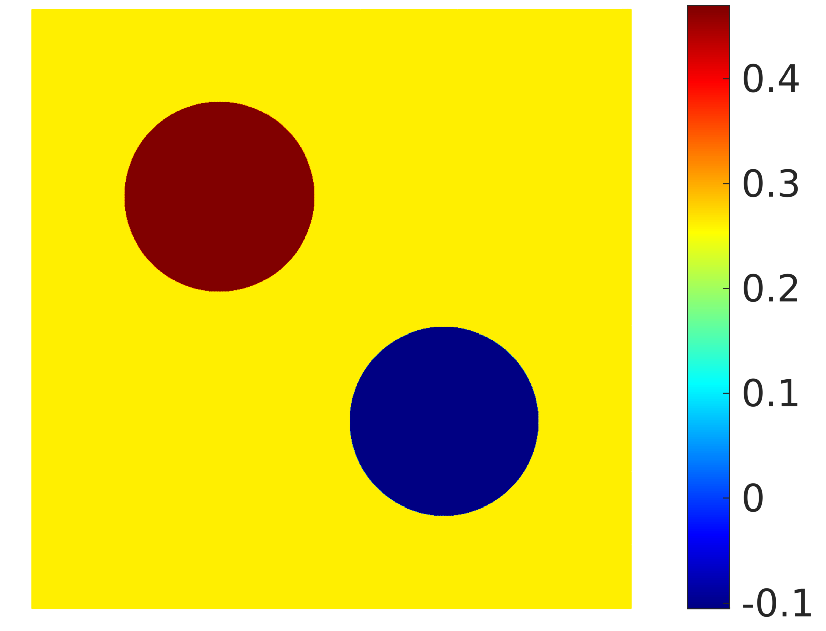
\includegraphics[width=0.7\textwidth]{Figures/sigma_exact}
	\end{minipage}
\end{frame}

\begin{frame}
\frametitle{Multiscale elliptic PDEs -- Inverse problems}
	\begin{figure}[t]
		\centering
		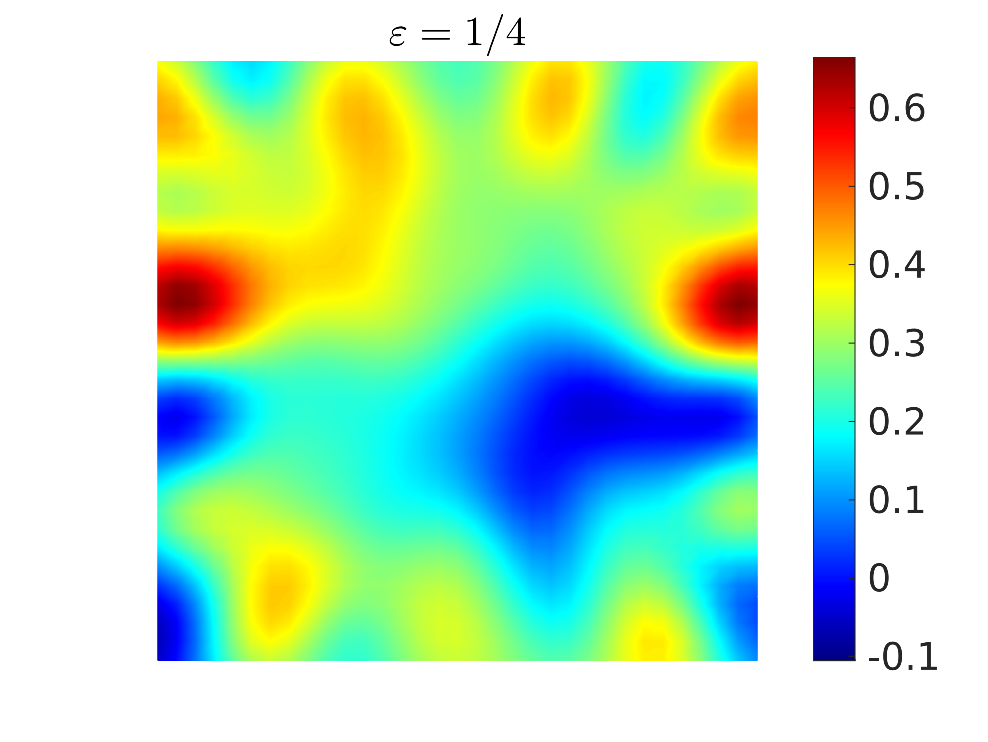
\includegraphics[width = 0.4\textwidth]{Figures/ensemble_500_e4}
		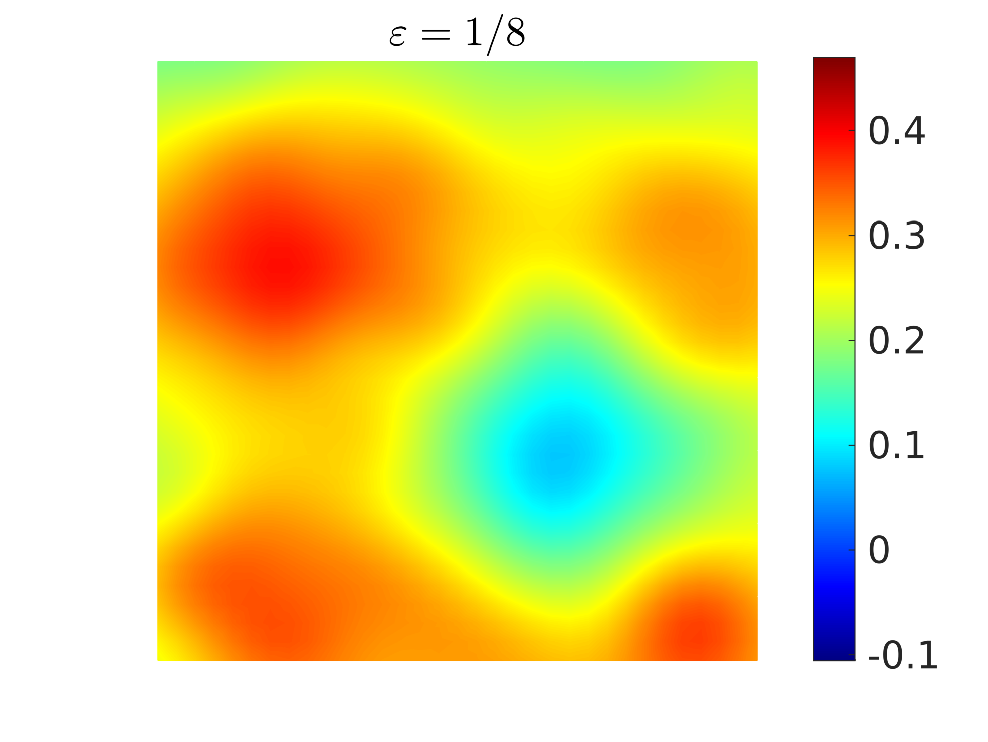
\includegraphics[width = 0.4\textwidth]{Figures/ensemble_500_e8}
		\\
		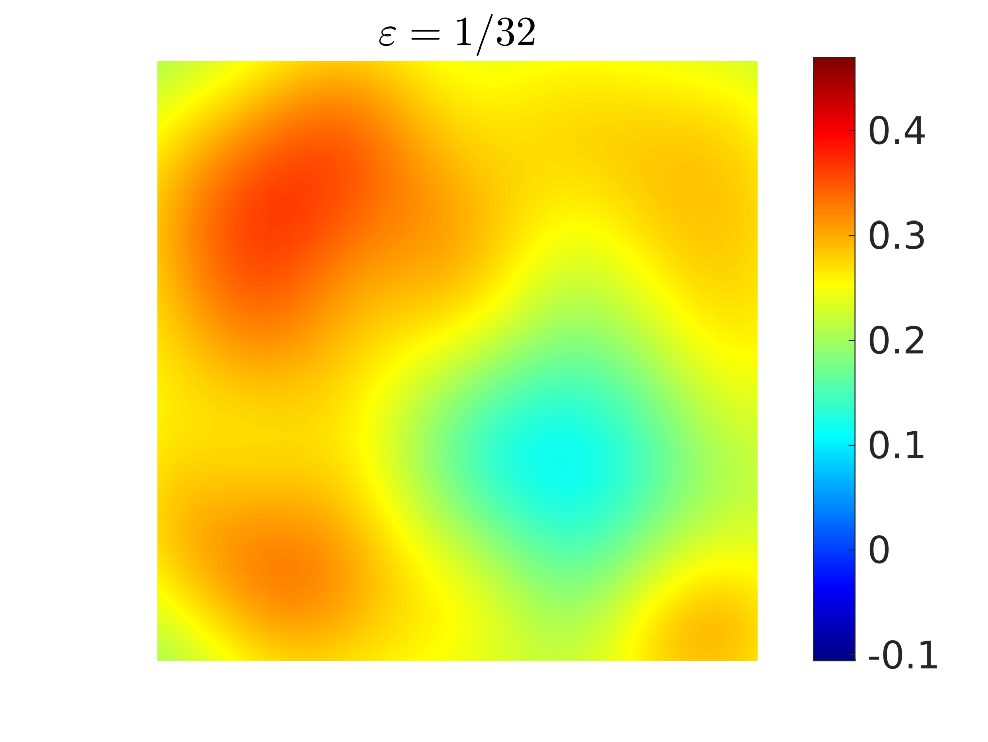
\includegraphics[width = 0.4\textwidth]{Figures/ensemble_500_e32}
		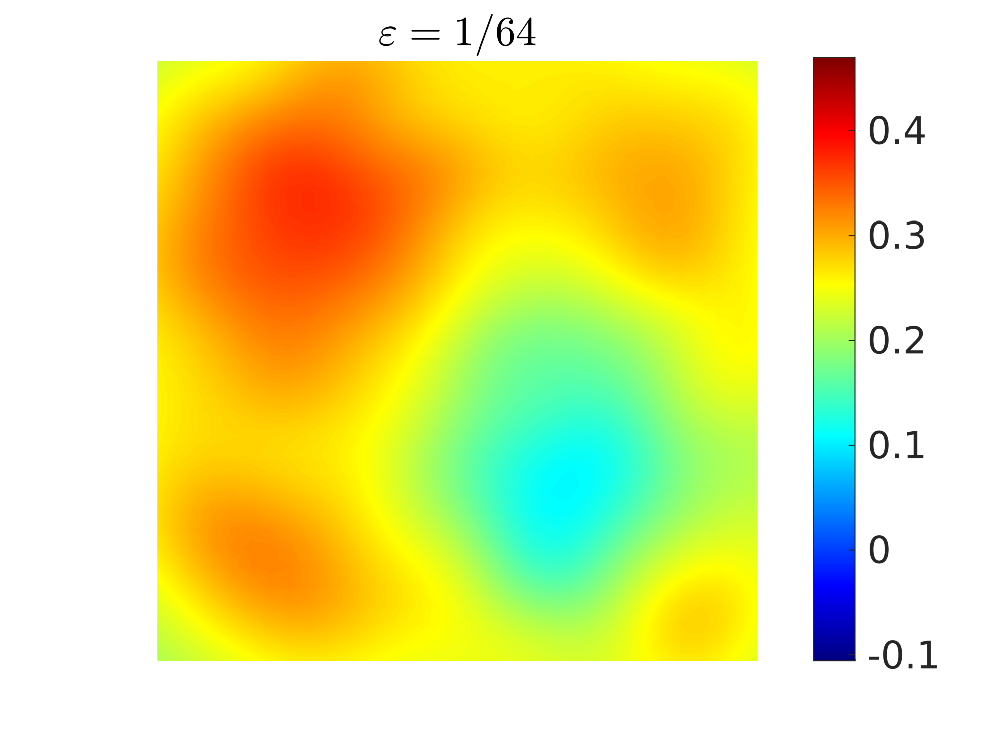
\includegraphics[width = 0.4\textwidth]{Figures/ensemble_500_e64}
		\caption{Convergence for $\epl \to 0$ of the EnKF posterior estimate.}
	\end{figure}
\end{frame}

\begin{frame}
\frametitle{Multiscale elliptic PDEs -- Inverse problems}
	
	{\color{BrickRed} Q2:} What if $\epl \ll 1$  (expensive) but $\epl$ far from asymptotic limit $\epl \to 0$?
	
	\vspace{0.5cm} 
	{\color{NavyBlue} Idea (\cite{CES14}):} Rewrite model as
	\begin{equation}
		y = \mathcal G^0_h(u) + m + \eta,
	\end{equation}
	where $m = \mathcal G^\epl(u) - \mathcal G^0_h(u)$ is the modelling error. Two approaches
	\begin{itemize}
		\item Assume $m \sim \mathcal N(\bar m, \bar \Sigma)$ independent of $\eta$, approximate offline from $\mu_{\mathrm{pr}}$
		\item Assume $m$ independent of $\eta$ and update distribution iteratively with a sequence of posterior distributions $\mu_l$, $l = 1, \ldots, L$
	\end{itemize}
	
	\vspace{0.3cm}
	{\color{BrickRed} Remark:} Modelling error approximation is crucial if $\epl$ small but ``not too small'': in this case we assume that it is possible to perform a limited number of evaluations of $\mathcal G^\epl$. 
\end{frame}

\begin{frame}
\frametitle{Multiscale elliptic PDEs -- Inverse problems}
	\begin{figure}[t]
		\centering
		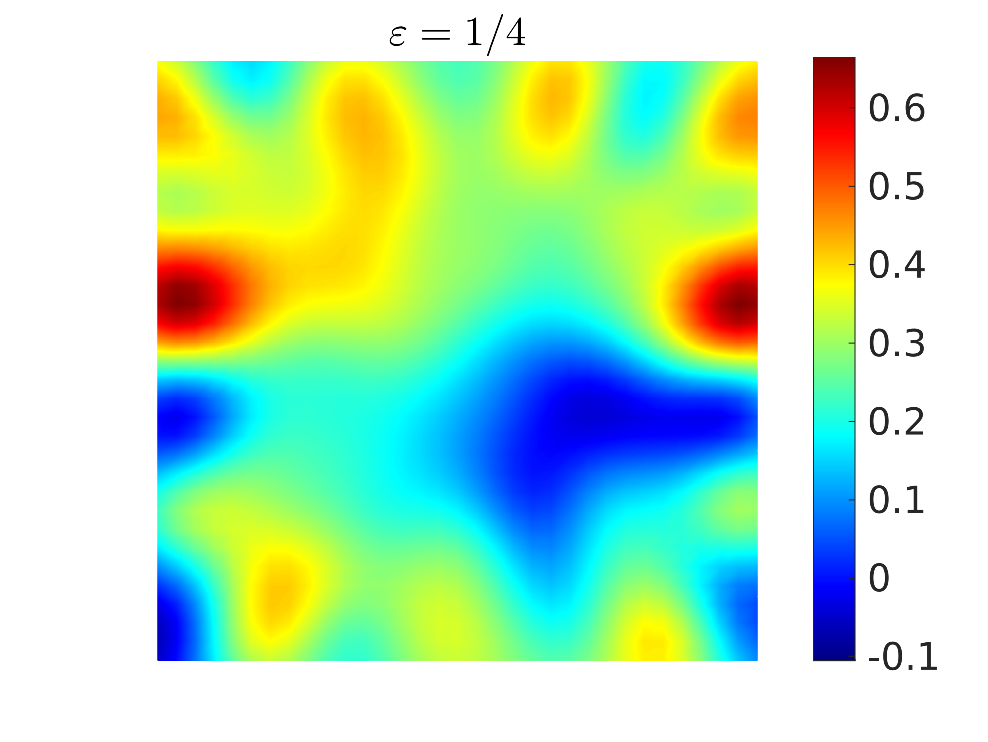
\includegraphics[width = 0.4\textwidth]{Figures/ensemble_500_e4}
		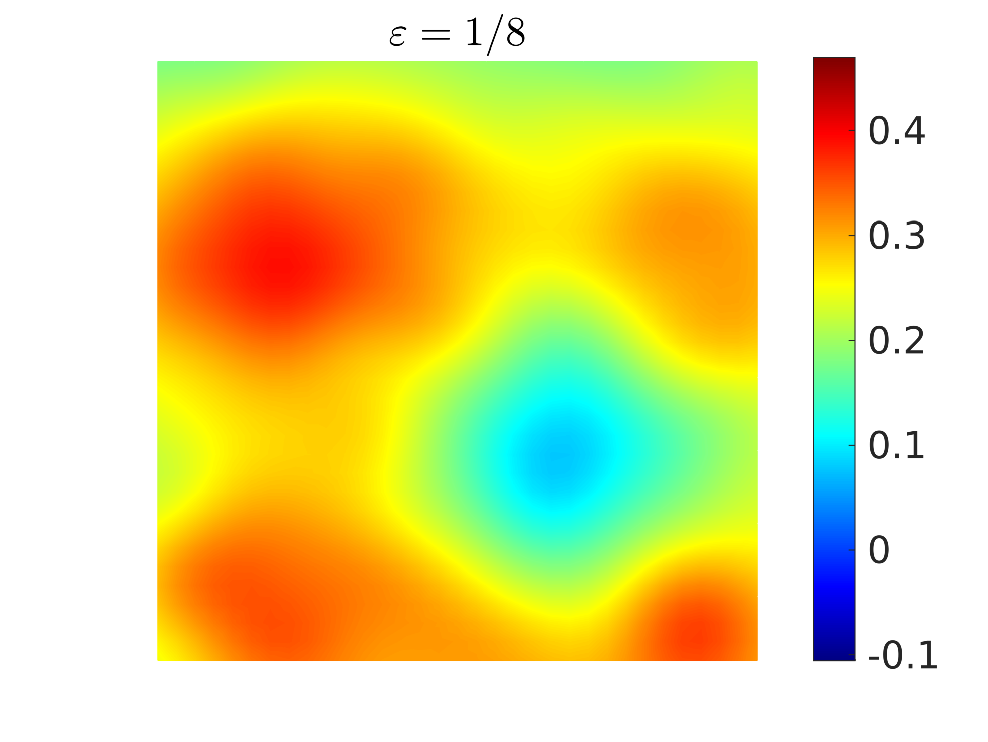
\includegraphics[width = 0.4\textwidth]{Figures/ensemble_500_e8}
		\\
		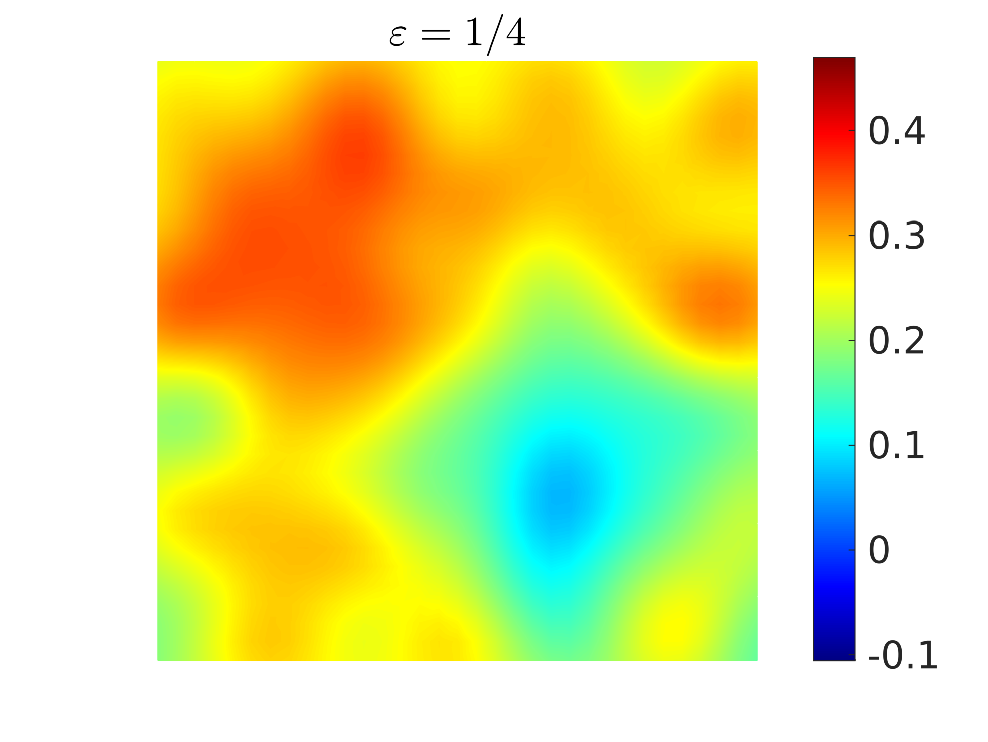
\includegraphics[width = 0.4\textwidth]{Figures/ensemble_500_e4_model_error}
		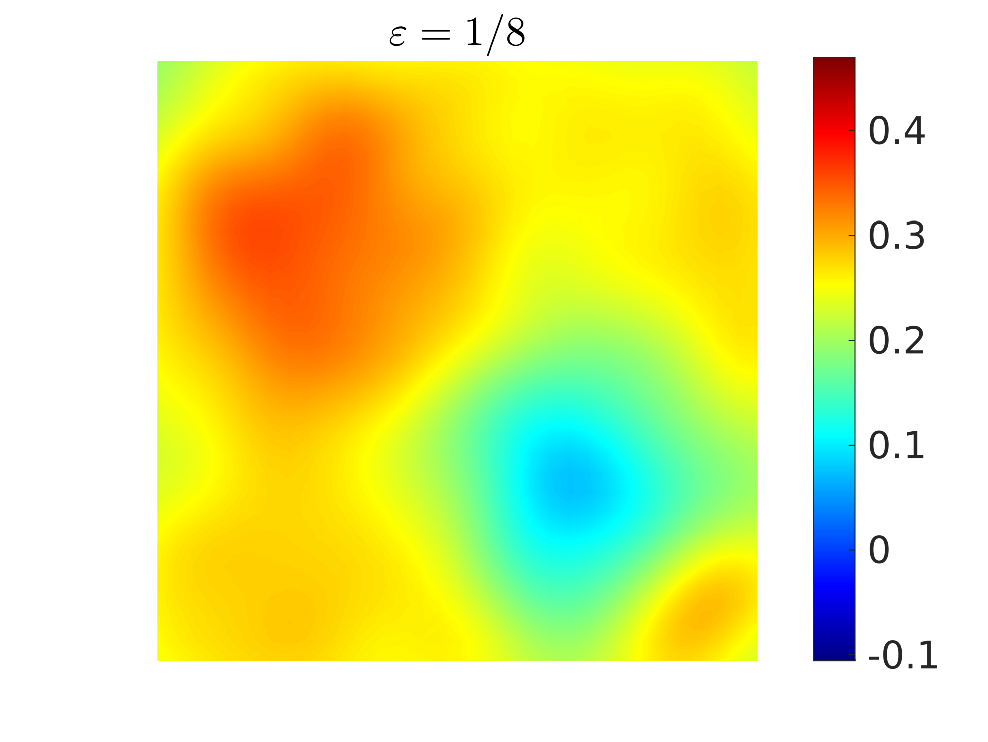
\includegraphics[width = 0.4\textwidth]{Figures/ensemble_500_e8_model_error}
		\caption{``Offline'' approximation of the modelling error.}
	\end{figure}
\end{frame}

\begin{frame}
\frametitle{Multiscale elliptic PDEs -- Inverse problems}
	\begin{figure}[t]
		\centering
		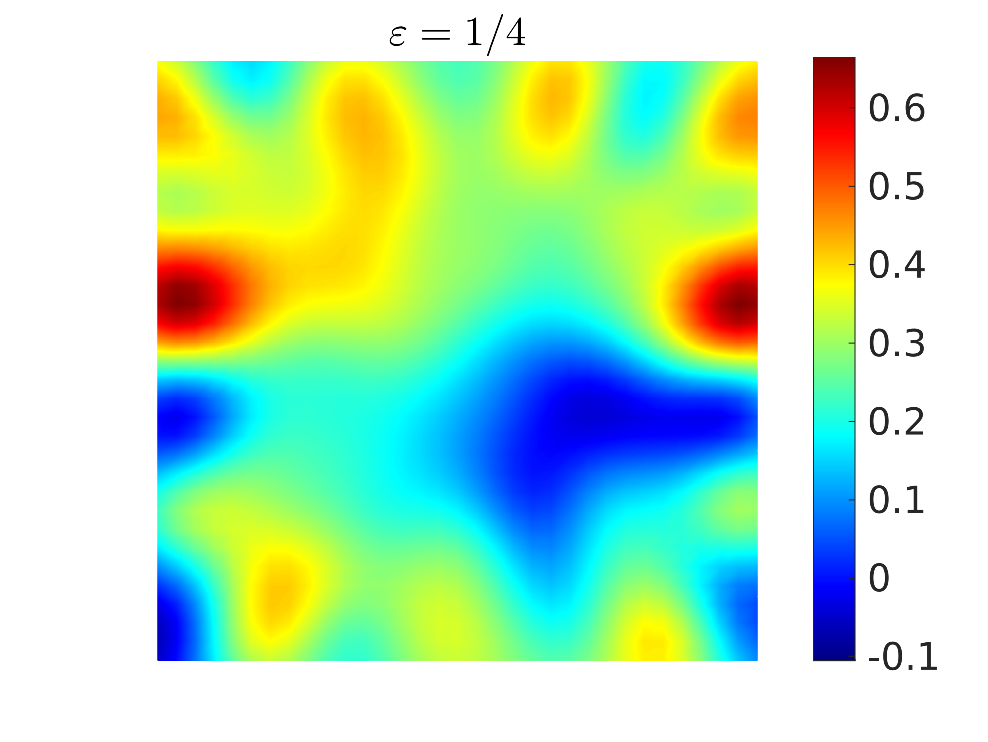
\includegraphics[width = 0.4\textwidth]{Figures/ensemble_500_e4}
		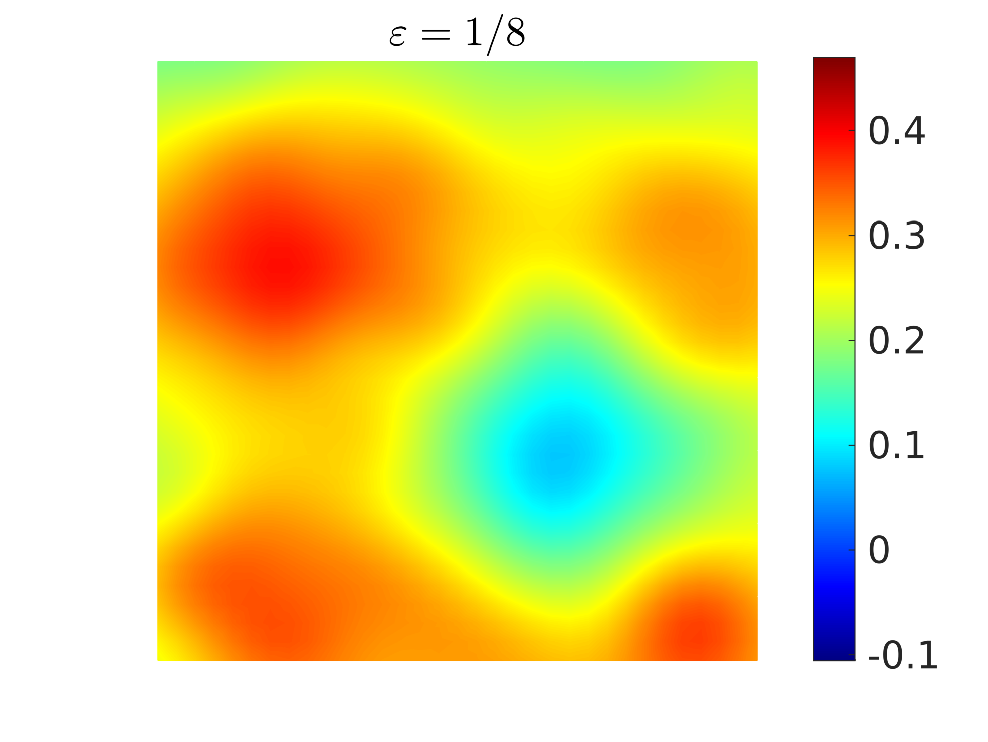
\includegraphics[width = 0.4\textwidth]{Figures/ensemble_500_e8}
		\\
		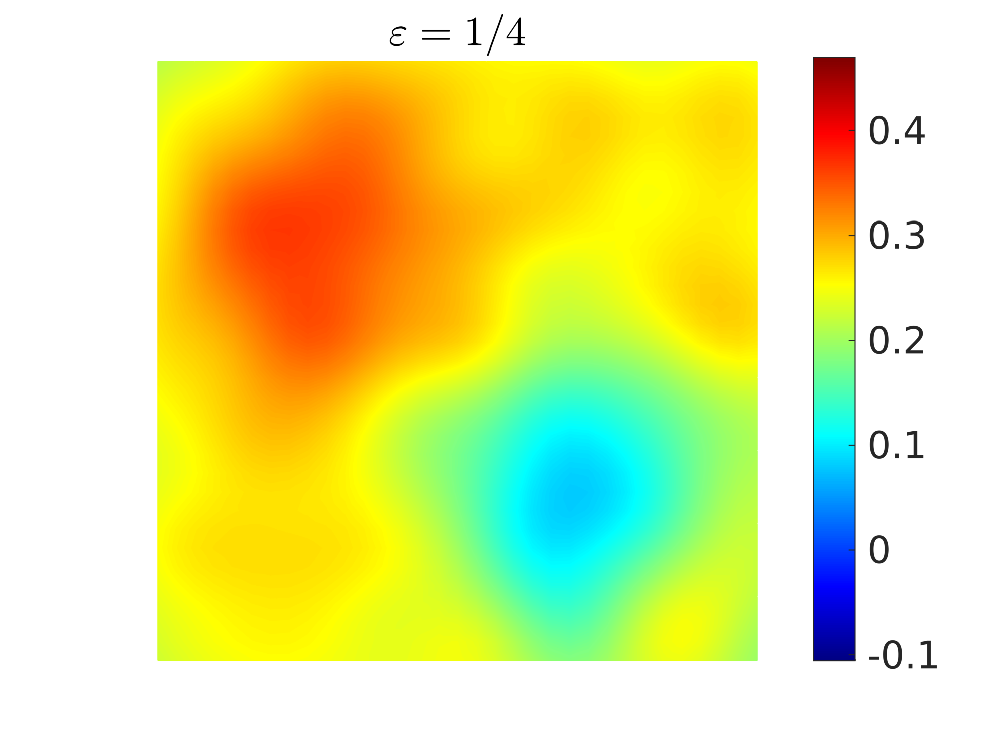
\includegraphics[width = 0.4\textwidth]{Figures/ensemble_500_e4_model_error_Levels}
		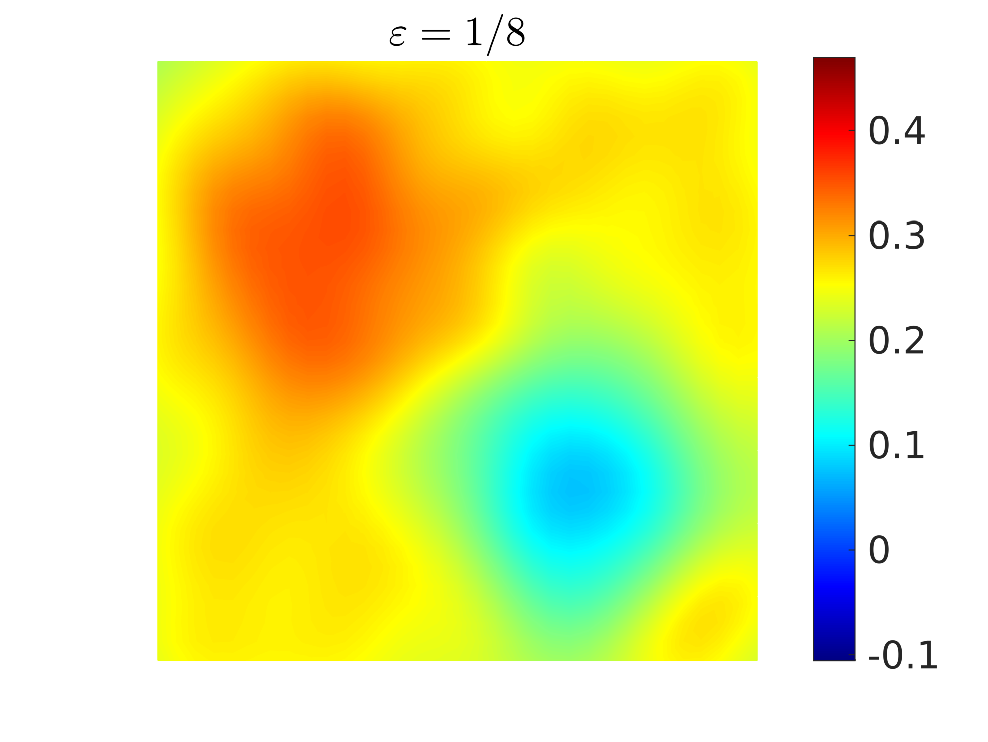
\includegraphics[width = 0.4\textwidth]{Figures/ensemble_500_e8_model_error_Levels}
		\caption{``Iterative'' approximation of the modelling error.}
	\end{figure}
\end{frame}

\subsection{Diffusion processes}

\begin{frame}
\frametitle{Multiscale diffusion processes}
	
	\onslide<1->
	Multiscale SDE -- first order Langevin
	\begin{equation}
		\dd x^\epl(t) = - \begingroup \color{ForestGreen} \underbrace{\vphantom{\frac{1}{\epl} \nabla V_1\Big(\frac{x^\epl(t)}{\epl}\Big)} \alpha \nabla V_0\big(x^\epl(t)\big) \dd t}_{\text{large-scale potential}} \endgroup 
						- \begingroup \color{BrickRed}    \underbrace{\frac{1}{\epl} \nabla V_1\Big(\frac{x^\epl(t)}{\epl}\Big)}_{\text{fluctuating potential}} \dd t\endgroup 
						+ \begingroup \color{NavyBlue}    \underbrace{\vphantom{\frac{1}{\epl} \nabla V_1\Big(\frac{x^\epl(t)}{\epl}\Big)} \sqrt{2\sigma} \dd W(t)}_{\text{diffusion}} \endgroup.
	\end{equation}

	\onslide<2-> {
	Homogenized SDE
	\begin{equation}
		\dd x^0(t) = - \begingroup \color{ForestGreen} A \, \nabla V_0 (x^0(t)) \dd t \endgroup 
					 + \begingroup \color{NavyBlue} \sqrt{2 \Sigma} \dd W(t) \endgroup,  \quad A = K\alpha, \, \Sigma = K \sigma.
	\end{equation}
	{\color{NavyBlue} Homogenization result (\cite{BLP78})}
	\begin{center}
		$x^\epl \Rightarrow x^0$ in $\mathcal C^0\big((0, T), \R^d\big)$ for $\epl \to 0$.
	\end{center}
	}	
\end{frame}

\begin{frameT}
\frametitle{Multiscale diffusion processes -- Inference problem}

	\vspace{0.5cm}
	{\color{NavyBlue} Inference problem}
	\begin{center} 
		Find $\theta = (\alpha, \sigma)$ given $\mathbf y = \mathbf x^\epl(\theta) + \boldsymbol \eta$, $\boldsymbol \eta \sim \rho_\eta$.
	\end{center}
	
	\only<1>{
	Posterior distribution $\mu^\epl(\theta \mid \mathbf y)$ with density
	\begin{equation}
		p^\epl(\theta \mid \mathbf y) = \frac{1}{Z^\epl} 
		\begingroup \color{ForestGreen} \underbrace{p(\theta)}_{\text{prior}} \endgroup \, 
		\begingroup \color{BrickRed} \underbrace{p^\epl(\mathbf y \mid \theta)}_{\text{likelihood}} \endgroup, 
		\quad Z^\epl \text{ s.t. } \int p^\epl(\theta \mid \mathbf y) \dd \theta = 1.
	\end{equation}
	
	{\color{ForestGreen} Prior}: Easy to evaluate (e.g. Gaussian), independent of $\epl$
	
	\vspace{0.3cm}
	{\color{BrickRed} Likelihood}: Needs more work
	}

	\only<2> {
	{\color{BrickRed} Likelihood}: Needs more work $\Rightarrow$ marginalization
	\begin{equation}
		{\color{BrickRed}	p^\epl(\mathbf y \mid \theta)} = \int_{\R^{Nd}} {\color{NavyBlue} p^\epl(\mathbf y \mid \mathbf x, \theta)} \, p^\epl(\mathbf x \mid \theta) \dd \mathbf x.
	\end{equation}
	where (observation independence)
	\begin{equation}
		{\color{NavyBlue} p^\epl(\mathbf y \mid \mathbf x, \theta) = \prod_{k=1}^N p^\epl(y_k \mid x_k, \theta)}.
	\end{equation}
	Observation density: $p(y_k \mid x_k, \theta) = \rho^{(k)}_\eta(y_k - x_k)$
	}

	\only<3> {
	{\color{BrickRed} Likelihood}: Needs more work $\Rightarrow$ marginalization
	\begin{equation}
	{\color{BrickRed}	p^\epl(\mathbf y \mid \theta)} = \int_{\R^{Nd}} {\color{NavyBlue} p(\mathbf y \mid \mathbf x, \theta)} \, p^\epl(\mathbf x \mid \theta) \dd \mathbf x.
	\end{equation}
	where (assume observation independence)
	\begin{equation}
	{\color{NavyBlue} p(\mathbf y \mid \mathbf x, \theta) = \prod_{k=1}^N p(y_k \mid x_k, \theta)}.
	\end{equation}
	Observation density: $p(y_k \mid x_k, \theta) = \rho^{(k)}_\eta(y_k - x_k)$ $\Rightarrow$ independent of $\epl$.
	}

	\only<4> {
	{\color{BrickRed} Likelihood}: Needs more work $\Rightarrow$ marginalization
	\begin{equation}
	{\color{BrickRed}	p^\epl(\mathbf y \mid \theta)} = \int_{\R^{Nd}} p(\mathbf y \mid \mathbf x, \theta) \, {\color{NavyBlue} p^\epl(\mathbf x \mid \theta)} \dd \mathbf x.
	\end{equation}
	where (Markov property)
	\begin{equation}
		{\color{NavyBlue} p^\epl(\mathbf x \mid \theta) = p(x_0) \prod_{k=1}^N p^\epl(x_k \mid x_{k-1}, \theta)}.
	\end{equation}
	\vphantom{Observation density: $p(y_k \mid x_k, \theta) = \rho^{(k)}_\eta(y_k - x_k)$ $\Rightarrow$ independent of $\epl$}Transition density: $p^\epl(x_k \mid x_{k-1}, \theta)$ $\Rightarrow$ only ``ingredient'' depending on $\epl$.
	}

	\only<5> {
	{\color{ForestGreen} Idea}: Replace  $p^0(\mathbf x \mid \theta) \approx p^\epl(\mathbf x \mid \theta)$ $\Rightarrow$ cheaper!
	
	\vspace{0.3cm}
	{\color{ForestGreen} Result}: Homogenized posterior $\mu^0(\theta \mid \mathbf y)$ with density  
	\begin{equation}
		p^0(\theta \mid \mathbf y) = \frac{1}{Z^0} 
		\begingroup \color{ForestGreen} p(\theta) \endgroup \, 
		\begingroup \color{BrickRed} p^0(\mathbf y \mid \theta) \endgroup, 
		\quad Z^0 \text{ s.t. } \int p^0(\theta \mid \mathbf y) \dd \theta = 1,
	\end{equation}
	with
	\begin{equation}
		{\color{BrickRed} p^0(\mathbf y \mid \theta)} = \int_{\R^{Nd}} p(\mathbf y \mid \mathbf x, \theta) \, p^0(\mathbf x \mid \theta) \dd \mathbf x.
	\end{equation}
	
	\vspace{0.2cm}
	{\color{BrickRed} Warning:} High-dimensional integral!
	}	

	\only<6>
	{
	{\color{ForestGreen} Idea}: Replace  $p^0(\mathbf x \mid \theta) \approx p^\epl(\mathbf x \mid \theta)$ $\Rightarrow$ cheaper!
	
	\vspace{0.3cm}
	{\color{ForestGreen} Result}: Homogenized posterior $\mu^0(\theta \mid \mathbf y)$ with density  
	\begin{equation}
	p^0(\theta \mid \mathbf y) = \frac{1}{Z^0} 
	\begingroup \color{ForestGreen} p(\theta) \endgroup \, 
	\begingroup \color{BrickRed} p^0(\mathbf y \mid \theta) \endgroup, 
	\quad Z^0 \text{ s.t. } \int p^0(\theta \mid \mathbf y) \dd \theta = 1,
	\end{equation}	
		
	{\color{NavyBlue} Theoretical result:} For $\epl \to 0$
	\begin{equation}	
		d_{\mathrm{Hell}}(\mu^\epl, \mu^0) \to 0.
	\end{equation}
	}
	
	\only<7>
	{
	{\color{NavyBlue} Theoretical result:} For $\epl \to 0$
	\begin{equation}	
	d_{\mathrm{Hell}}(\mu^\epl, \mu^0) \to 0.
	\end{equation}
	
	\vspace{0.5cm}
	{\color{BrickRed} Questions (Recall):} 
	
	{\color{BrickRed} Q1:}  Does approximating $\mu^0$ spoil multiscale convergence?
	
	{\color{BrickRed} Q2:} What if $\epl \ll 1$  (expensive) but $\epl$ far from asymptotic limit $\epl \to 0$?
	}

	\only<8>
	{
		{\color{NavyBlue} Theoretical result:} For $\epl \to 0$
		\begin{equation}	
		d_{\mathrm{Hell}}(\mu^\epl, \mu^0) \to 0.
		\end{equation}
		
		\vspace{0.5cm}
		{\color{BrickRed} Questions ($\approx$ Recall):} 
		
		{\color{BrickRed} Q1:}  How do we sample from $\mu^0$?
		
		{\color{BrickRed} Q2:} What if $\epl \ll 1$  (expensive) but $\epl$ far from asymptotic limit $\epl \to 0$?
	}
\end{frameT}

\begin{frameT}
\frametitle{Multiscale diffusion processes -- Inference problem}

{\color{BrickRed} Q1:}  How do we sample from $\mu^0$?
\vspace{0.4cm}

\only<1-2>{
{\color{NavyBlue} Recall:} Density of $\mu^0(\theta \mid \mathbf y)$ 
\begin{equation}
p^0(\theta \mid \mathbf y) = \frac{1}{Z^0} 
\begingroup \color{ForestGreen} p(\theta) \endgroup \, 
\begingroup \color{BrickRed} p^0(\mathbf y \mid \theta) \endgroup, 
\quad Z^0 \text{ s.t. } \int p^0(\theta \mid \mathbf y) \dd \theta = 1,
\end{equation}	
with
\begin{equation}
{\color{BrickRed} p^0(\mathbf y \mid \theta)} = \int_{\R^{Nd}} p(\mathbf y \mid \mathbf x, \theta) \, p^0(\mathbf x \mid \theta) \dd \mathbf x.
\end{equation}
}

\only<2>{
\vspace{0.1cm}
{\color{NavyBlue} Solution:} Employ a particle filter (PF) to obtain an estimator
\begin{equation}
\begin{aligned}
	\widehat{p^0}(\theta \mid \mathbf y) &= p(\theta) \, \widehat{p^0}(\mathbf y \mid \theta) \approx p^0(\theta \mid \mathbf y), \\
	\E\widehat{p^0}(\theta \mid \mathbf y) &= p^0(\theta \mid \mathbf y),
\end{aligned}
\end{equation}
then run a particle MCMC (PMCMC) algorithm (\cite{ADH10})
}

\only<3> {
{\color{NavyBlue} PMCMC:} Given $\theta^{(0)}$, $M \in \mathbb N$, proposal $q$

\begin{enumerate}
	\item compute $\widehat p^{(0)} = \widehat p(\theta^{(0)} \mid \mathbf y)$
	\item For $k = 0, \ldots, M$
	\begin{enumerate}
		\item sample $\theta^\star \sim q(\cdot \mid \theta^{(k)})$
		\item compute $\hat p^\star = \hat p(\theta^\star \mid \mathbf y)$
		\item 	compute $$\alpha\big(\theta^*, \theta^{(k)}\big) = \min\Big\{1, \frac{\hat p^\star}{\hat p^{(k)}} \, \frac{q(\theta^{(k)} \mid \theta^\star)}{q(\theta^\star \mid \theta^{(k)})}\Big\};$$ 
		\item 	with probability $\alpha\big(\theta^\star, \theta^{(k)}\big)$ set $\theta^{(k+1)} = \theta^\star$, $\hat p^{(k+1)} = \hat p^\star$, 	otherwise set $\theta^{(k+1)} = \theta^{(k)}$, $\hat p^{(k+1)} = \hat p^{(k)}$
	\end{enumerate}
\end{enumerate}

\vspace{0.2cm}
{\color{NavyBlue} Property:} PF likelihood estimator unbiased $\implies$ PMCMC targets the correct posterior
}
\end{frameT}

\begin{frame}
\frametitle{Multiscale diffusion processes -- Inference problem}

\onslide<1->{
{\color{BrickRed} Q2:} What if $\epl \ll 1$  (expensive) but $\epl$ far from asymptotic limit $\epl \to 0$?

\vspace{0.3cm}
{\color{NavyBlue} Modelling error:} Same idea as in the PDE case
\begin{equation}
	\mathbf y = \mathbf x^0(\theta) + \mathbf m + \mathbf \eta,
\end{equation}
where $\mathbf m \coloneqq \mathbf x^\epl - \mathbf x^0$. We can assume $\mathbf m$ independent of $\eta$ and $\theta$, and compute the likelihood consequently with offline or dynamic procedures.
}

\onslide<2->{
\vspace{0.1cm}
{\color{NavyBlue} Idea (latest):} Use PF for estimation of modelling error on state
\begin{equation}
	\mathbf X \coloneqq (\mathbf x^\epl, \, \mathbf m)^\top,
\end{equation}
for which we have dynamics (neglect correlation)
\begin{equation}
\left\{
\begin{alignedat}{2}
	X_{k+1} &\sim \begin{pmatrix} p(x^\epl \mid x^\epl_k) \\ p(m \mid m_k)\end{pmatrix}, &&\quad \text{(transition)}, \\
	y_{k+1} &= H X_{k+1} + \eta_{k+1}, &&\quad \text{(observation)}
\end{alignedat}
\right.
\end{equation}
where $H = (I, \, 0)^\top$.
}	
\end{frame}

\begin{frame}
\frametitle{Multiscale diffusion processes -- Inference problem}

{\color{NavyBlue} Numerical experiment (setting from \cite{PaS07}):} 

\vspace{0.2cm}
Consider one-dimensional multiscale SDE
\begin{equation}
	\d x^\epl(t) = -\alpha x^\epl(t) \dd t +\frac{1}{\epl} \sin\left(\frac{x^\epl}{\epl}\right) + \sqrt{2\sigma} \d W(t),
\end{equation}
with $\epl = 0.1$ and $\alpha = 1$, $\sigma = 0.5$. In this case
\begin{equation}
	\d x^0(t) = -A x^0(t) \dd t + \sqrt{2\Sigma} \d W(t),
\end{equation}
where
\begin{equation}
	\Sigma = \frac{4\sigma\pi^2}{Z \widehat Z}, \quad A = \frac{4\alpha\pi^2}{Z \widehat Z},
\end{equation}
and
\begin{equation}
	Z = \int_0^{2\pi} e^{-\cos(y)/\sigma} \dd y, \quad \widehat Z = \int_0^{2\pi} e^{\cos(y)/\sigma} \dd y.
\end{equation}

\vspace{0.2cm}
{\color{NavyBlue} Goal:} Determine posterior over $(\alpha, \sigma)$ employing homogenized model.
\end{frame}

\begin{frame}
\frametitle{Multiscale diffusion processes -- Inference problem}
\begin{figure}[t]
	\centering
	\includegraphics[width = 0.45\textwidth]{Figures/MultiMulti}
	\includegraphics[width = 0.45\textwidth]{Figures/MultiHomo}
	\caption{Parameter estimation without and with (iterative) estimation of modelling error.}
\end{figure}

\end{frame}

\appendix
\begin{frame}[allowframebreaks]{References}

\bibliographystyle{apalike}
\begin{scriptsize}
	\bibliography{../anmc}
\end{scriptsize}


\end{frame}

\end{document}
